\documentclass{article}
\usepackage{apacite}
\usepackage{blindtext}
\usepackage{amsmath}
\usepackage{amssymb}
\usepackage{amsmath}
\usepackage[utf8]{inputenc}
\usepackage{bbm}
\usepackage[margin=1in]{geometry} % set margins
\usepackage{subcaption} % allows for subfigures
\usepackage{graphicx} % allow inclusion of figures/photos/pdfs
\usepackage{setspace} % allows changes between 
% \doublespacing \singlespacing \onehalfspacing
\onehalfspacing
\graphicspath{{./figure/}}
\usepackage[justification=centering]{caption}
\usepackage{cancel}
\usepackage{mathrsfs}

\usepackage{Sweave}
\begin{document}
\Sconcordance{concordance:Dilgin_MPSA.tex:Dilgin_MPSA.Rnw:%
1 19 1 1 0 133 1 1 11 31 1}

	\title{Where to Spend the Money? A Survey Experiment on Electoral Institutions and Party Expenditure at the District Level}
	\author{Tolgahan Dilgin}
	\date{03/28/2018}
	\maketitle
	
\begin{abstract}
This paper is part of dissertation research that examines the impact of electoral institutions on how political parties choose to engage in vote buying practices at the district level. Regardless of electoral rules, parties tend to concentrate their vote buying spending in the most competitive districts as opposed to party strongholds in order to maximize their electoral gains. This research argues that Proportional Representation (PR) systems enable political parties distribute their vote buying activities more evenly between party strongholds and competitive districts in comparison to Single Member District (SMD) systems. In the face of difficulty in testing this theory empirically, the paper takes advantage of the unique political structure of Mexico, which uses both SMD and PR systems in its elections. The survey experiment with Mexican students -who are exposed to both of the systems- seems to provide evidence consistent with paper's main theoretical claim.
\end{abstract}

\section{Introduction}
The consequences of electoral systems have been a widely debated topic in political science for several decades. The argument that Proportional Representtion performs better on several aspects of democratic life goes back to John Stuart Mill's \cite{mill1861considerations} The reason for and consequences of several European countries' shift from Single Member District (SMD) system to Proportional Representation in Europe was a theme that was discussed in the 1970s \cite{rokkan_citizens_1970}. Ever since, the scholarly work has made important advances on our knowledge on how electoral institutions may help us explain certain political phenomena. Perhaps, our most widely accepted piece of knowledge is about the existent trade of between representation and accountability \cite{diamond1999developing}.



\iffalse the tradeoff
Matt's PS 345 slide. 
Electoral System Design: Four Normative Tradeoffs (Diamond 1999)
-Efficiency/Governability vs. Representativeness
-Representativeness/Inclusiveness vs. Vertical Accountability/Accessibility 
-Party Coherence vs. Voter Choice
- Simplicity/Ballot Accessibility vs. Appropriateness of System to Country

--
Actual, Diamond 1999- Developing Democracy: Toward Consolidation p.100
"Four normative trade-offs become salient in designing (or reforming) electoral systems for contemporary democracies"
Efficiency \& governability vs. representativeness
"The more majoritarian the electoral system, the greater the distortion (disproportionality) between votes and seats, and the less representative the outcome (in giving parliamentary place voice to all interests and views.) However, the efficiency of democracy, "the ability of elections to serve as a means for voters to identify and choose among the competing government options available," is best served with a majoritarian electoral system, which can provide coherent governing alternatives known to the electorate in advance (ideally between two parties) and also a governing majority (footnote 94)."

Representativeness \& inclusiveness (PR) vs. direct vertical accountability \& accessibility (SMD system)

\fi



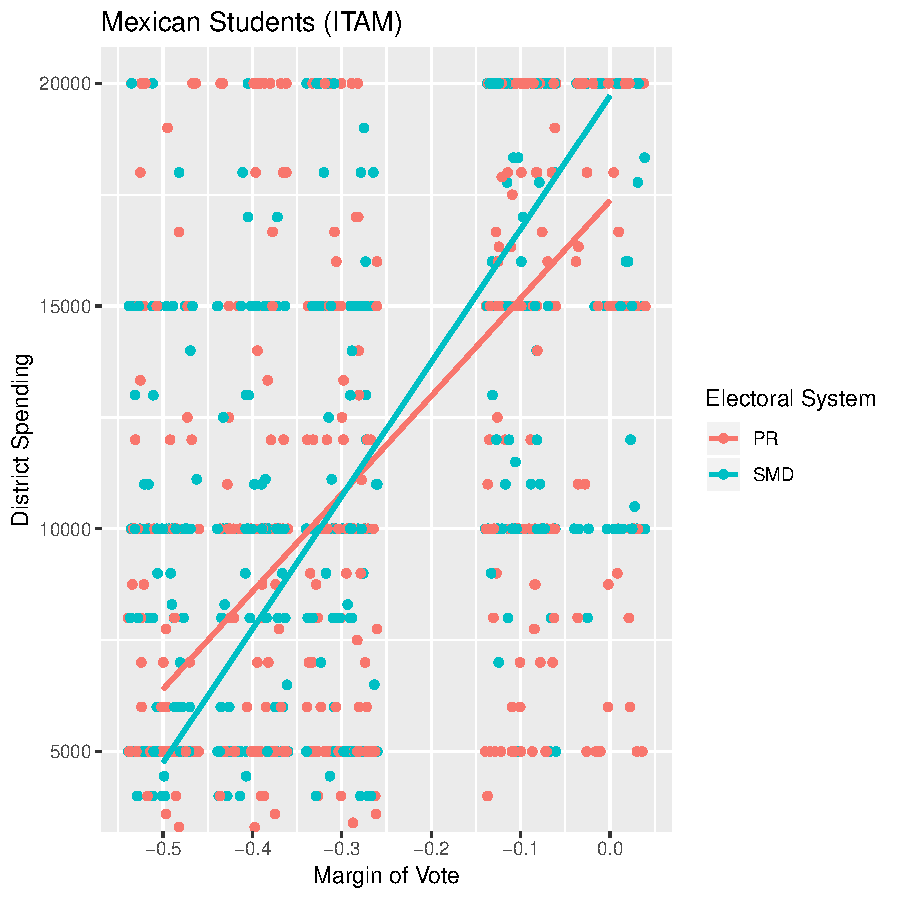
\includegraphics{Dilgin_MPSA-002}




\bibliographystyle{apacite}
\bibliography{MPSA_References}

\end{document}
